\documentclass[conference]{IEEEtran}
\IEEEoverridecommandlockouts
% The preceding line is only needed to identify funding in the first footnote. If that is unneeded, please comment it out.
\usepackage{cite}
\usepackage{amsmath,amssymb,amsfonts}
\usepackage{algorithmic}
\usepackage{graphicx}
\usepackage{textcomp}
\usepackage{xcolor}
\usepackage{tabularx}
\usepackage{multirow}
\usepackage{graphics} % for pdf, bitmapped graphics files
\usepackage{subfig}
\usepackage{subcaption}
\usepackage{hyperref}
\usepackage{academicons}
\usepackage{xcolor}
\usepackage{listings}
\usepackage{tabularx} % Asegúrate de incluir este paquete

\usepackage{tikz}
\usetikzlibrary{shapes.geometric, arrows}

\usetikzlibrary{shapes.geometric, arrows}

\tikzstyle{startstop} = [rectangle, rounded corners, minimum width=3cm, minimum height=1cm,text centered, draw=black, fill=red!30]
\tikzstyle{process} = [rectangle, minimum width=3cm, minimum height=1cm, text centered, draw=black, fill=blue!30]
\tikzstyle{arrow} = [thick,->,>=stealth]


\def\BibTeX{{\rm B\kern-.05em{\sc i\kern-.025em b}\kern-.08em
		T\kern-.1667em\lower.7ex\hbox{E}\kern-.125emX}}

% Color Enlace
\definecolor{colorEnlace}{RGB}{0, 0, 0}
\hypersetup{
	colorlinks=true,
	linkcolor=colorEnlace,
	citecolor=colorEnlace,
	urlcolor=colorEnlace,
	pdfauthor={Davis Bremdow Salazar Roa},
	pdftitle={Sistemas Embebidos}
}
\definecolor{mybg}{rgb}{0.97,0.97,0.97}
\definecolor{mygray}{gray}{0.4}
\definecolor{mygreen}{rgb}{0,0.6,0}
\definecolor{myblue}{rgb}{0,0,0.8}
\definecolor{mypurple}{rgb}{0.58,0,0.82}
\definecolor{myred}{rgb}{0.7,0,0}

\lstdefinelanguage{MatlabEnhanced}{
	language=Matlab,
	morekeywords={[2]linspace,plot,title,xlabel,ylabel,legend,grid},
	morekeywords={[3]sin,cos,exp,log,sqrt},
	keywordstyle=\color{myblue}\bfseries,
	keywordstyle=[2]\color{mypurple},
	keywordstyle=[3]\color{myred},
	commentstyle=\color{mygreen}\itshape,
	stringstyle=\color{mygray},
	morecomment=[l]%
}

\lstset{
	language=MatlabEnhanced,
	backgroundcolor=\color{mybg},
	frame=single,
	basicstyle=\ttfamily\small,
	showstringspaces=false,
	numbers=none,              %
	xleftmargin=0pt,           %
	framexleftmargin=0pt,      
	framexrightmargin=0pt,
	framextopmargin=2pt,
	framexbottommargin=2pt,
	breaklines=true,
	tabsize=1,
}

% Control 
\usepackage{amsmath}
\begin{document}
	
	\title{Análisis de Ruido en una señal FM}
	\author{
		\makebox[\textwidth][c]{\large\textbf{Universidad Nacional de San Antonio Abad del Cusco}}\\
		\makebox[\textwidth][c]{\normalsize\textit{Escuela profesional de Ingeniería Electrónica}}\\
		\makebox[\textwidth][c]{\normalsize\textit{Ing. Milton Velasquez curo}}\\
		\makebox[\textwidth][c]{\normalsize\textit{Telecomunicaciones I}}\\
		\and
		\IEEEauthorblockN{Ruth Juana Espino Puma - 185746}
		\IEEEauthorblockA{Estudiante de Ingeniería Electrónica \\
			Cusco, Perú \\
			184657@unsaac.edu.pe}
		\and
		\IEEEauthorblockN{Aaron Quispe Coyla - 200832}
		\IEEEauthorblockA{Estudiante de Ingeniería Electrónica \\
			Cusco, Perú \\
			200832@unsaac.edu.pe}
		\and
		\IEEEauthorblockN{Davis Bremdow Salazar Roa - 200353}
		\IEEEauthorblockA{Estudiante de Ingeniería Electrónica \\
			Cusco, Perú \\
			200353@unsaac.edu.pe}
		
	}
	
	\maketitle
	\begin{abstract}
		
	\end{abstract}
	
	\begin{IEEEkeywords}
		Modulación FM, SNR
	\end{IEEEkeywords}
	
	%% Contenido del documento
	\section{ SNR en la demodulación FM}
	
	La SNR en FM se define como la relación entre la potencia media de la señal modulada y la potencia media del ruido en una portadora sin modular, implicando que el ruido en la señal moduladora no influye significativamente en este tipo de esquema.
	
	
	
	\section{ Metodología }
	
	Para poder cuantizar la influencia del generador de ruido en la demodulación FM, es de vital importancia poder modificar los parámetros de una señal FM, siendo que dentro de ello se debe considerar, el ancho de banda de la señal de información, la desviación máxima estándar y en función a ello el índice de modulación, además para poder trabajar dentro del ancho de banda de influencia del dispositivo de ruido también fue necesario controlar la frecuencia de transmisión.
	
	En tal sentido para este propósito se definieron 2 proyectos en el software GNU Radio que constituyen a un transmisor y demodulador FM los cuales pudieron facilitar la variación de parámetros.
	
	\subsection{ Transmisor FM }
	
	En la parte del transmisor FM se definió una modulación WBFM (Wide Band FM) esto con la finalidad de poder modificar el valor de $\beta$ o índice de modulación en el intervalo entre 0 y 10, en la figura \ref{fig:transmisor-fm} se muestra un esquema gráfico para este propósito en el cual para la transmisión se hace uso del bloque WBFM el cual internamente realiza el proceso de mezclado para la generación de una señal FM,, además también se hicieron uso  2
	
	
	\begin{figure}[h]
		\centering
		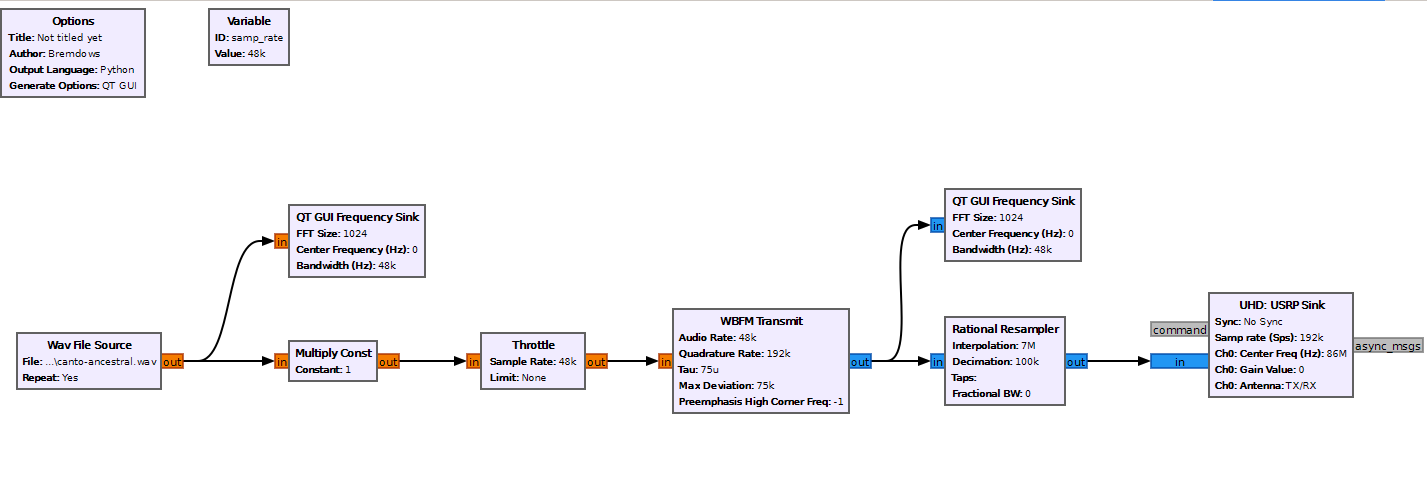
\includegraphics[width=0.5\textwidth]{media/transmisor-fm}
		\caption{SDR: Transmisor FM - GNU Radio}
		\label{fig:transmisor-fm}
	\end{figure}
	
	
	\subsection{ Receptor FM }
	
	El bloque receptor FM, se considero como elemento de validación de frecuencia y potencia de la señal transmitida, este a su vez estuvo compuesto por un bloque de entrada o de recepción perteneciente al USRP 2910 / 2920, un bloque para modifica la tasa de muestreo (Rational Resampler) para luego conectar estas 2 etapas previas con el bloque de demodulación FM (WBFM Receive), finalmente debido a la alta tasa de muestreo en la recepción al momento de reproducir la señal sintonizada, fue necesario volver a modificar la tasa de muestreo para adecuarla al estándar de 48k [Hz].
	
	\begin{figure}[h]
		\centering
		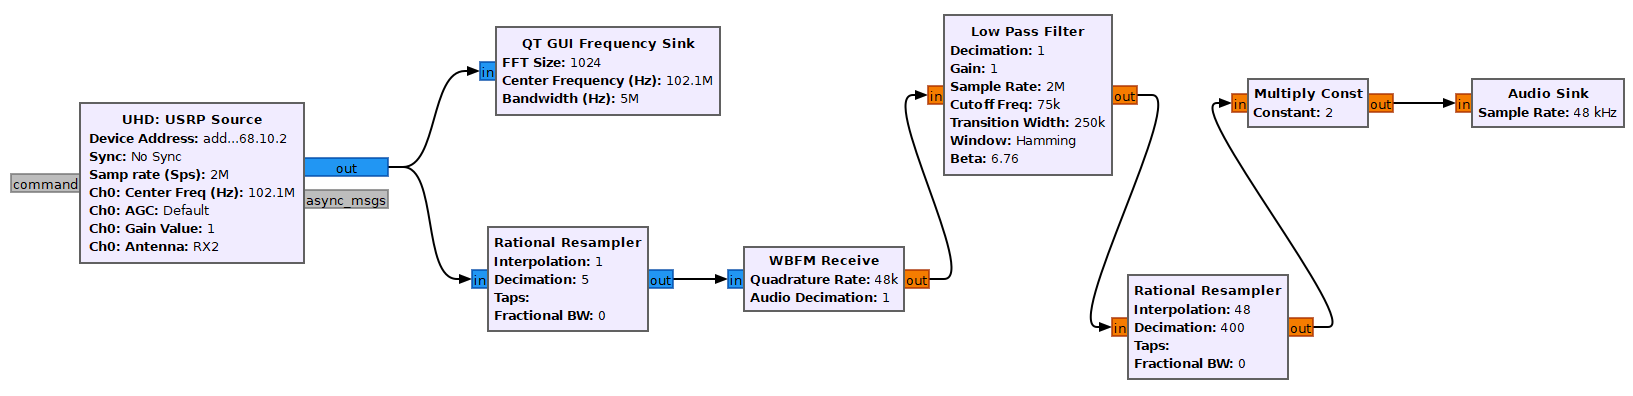
\includegraphics[width=0.5\textwidth]{media/receptor-fm}
		\caption{Receptor FM - GNU Radio}
		\label{fig:receptor-fm}
	\end{figure}
	
	En la figura \ref{fig:receptor-fm} se muestra el esquema general de los bloques utilizados en GNU Radio, además se debe tener en cuenta
	
	\subsection{ Estimación del piso de ruido }
	
	Para el procesamiento de las mediciones obtenidos en formato .csv, se hizo uso del entorno matricial MATLAB, esto debido a su facilidad para el tratamiento de datos en forma de arreglos y al contar con herramientas de navegación entre directorios, permitió automatizar la lectura, tratado y modificación de los datos medidos.
	
	Para tener una coherencia entre el tratado de datos y los resultados obtenidos, fue necesario categorizar mediante una etiqueta y/o nombre de archivo (cada medición) ello con la finalidad de especificar una determinada distancia, tipo de medición y parámetros configurados en la transmisión FM, para ello se uso:
	
	\begin{itemize}
		\item R[distancia en metros]: Para referirse a una señal compuesta solo por ruido.
		\item SR[consonante][distancia]\_Beta: Define una señal FM transmitida con ruido para un beta determinado.
		\item TPR: Refiere al piso de ruido sin ninguna interferencia provocada.
	\end{itemize}
	
	En la figura \ref{fig:jerarquia-archivos} se puede apreciar el esquema general y la jerarquía de archivos resultante para el procesamiento.
	
	\begin{figure}[h]
		\centering
		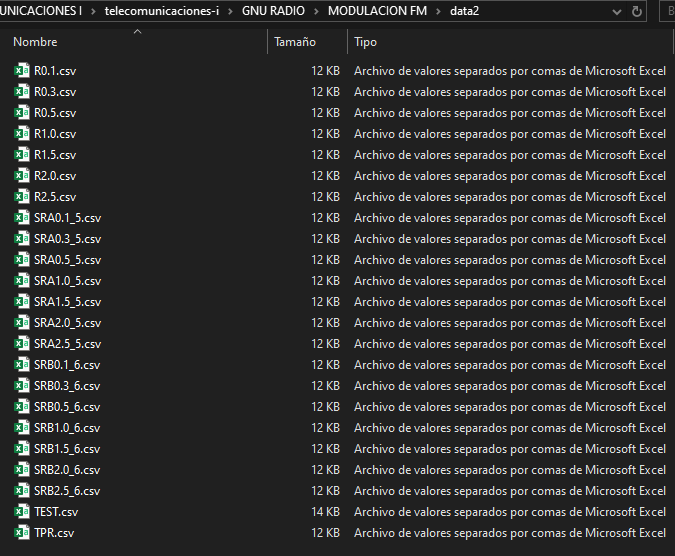
\includegraphics[width=0.5\textwidth]{media/jerarquia-archivos}
		\caption{Jerarquía de Archivo - Procesamiento}
		\label{fig:jerarquia-archivos}
	\end{figure}
	
	
	El piso de ruido esta compuesto por diferentes señales que perturban su medición, como se muestra en la figura \ref{fig:piso-ruido} esta parámetro es de carácter no determinista siendo así que obtener un valor directo es inexacto, por lo que se empleo la obtención de la media entre los valores medidos para obtener un valor representativo que nos permita cuantificar, sin embargo la existencia de los picos (valores extremos) alteran esta medida al desplazar el valor de la media, por lo tanto para evitar este inconveniente, se hace uso de una función limitadora de picos, la cual elimina los valores por fuera de un rango especifico, para facilitar las mediciones.
	
	\begin{figure}[h]
		\centering
		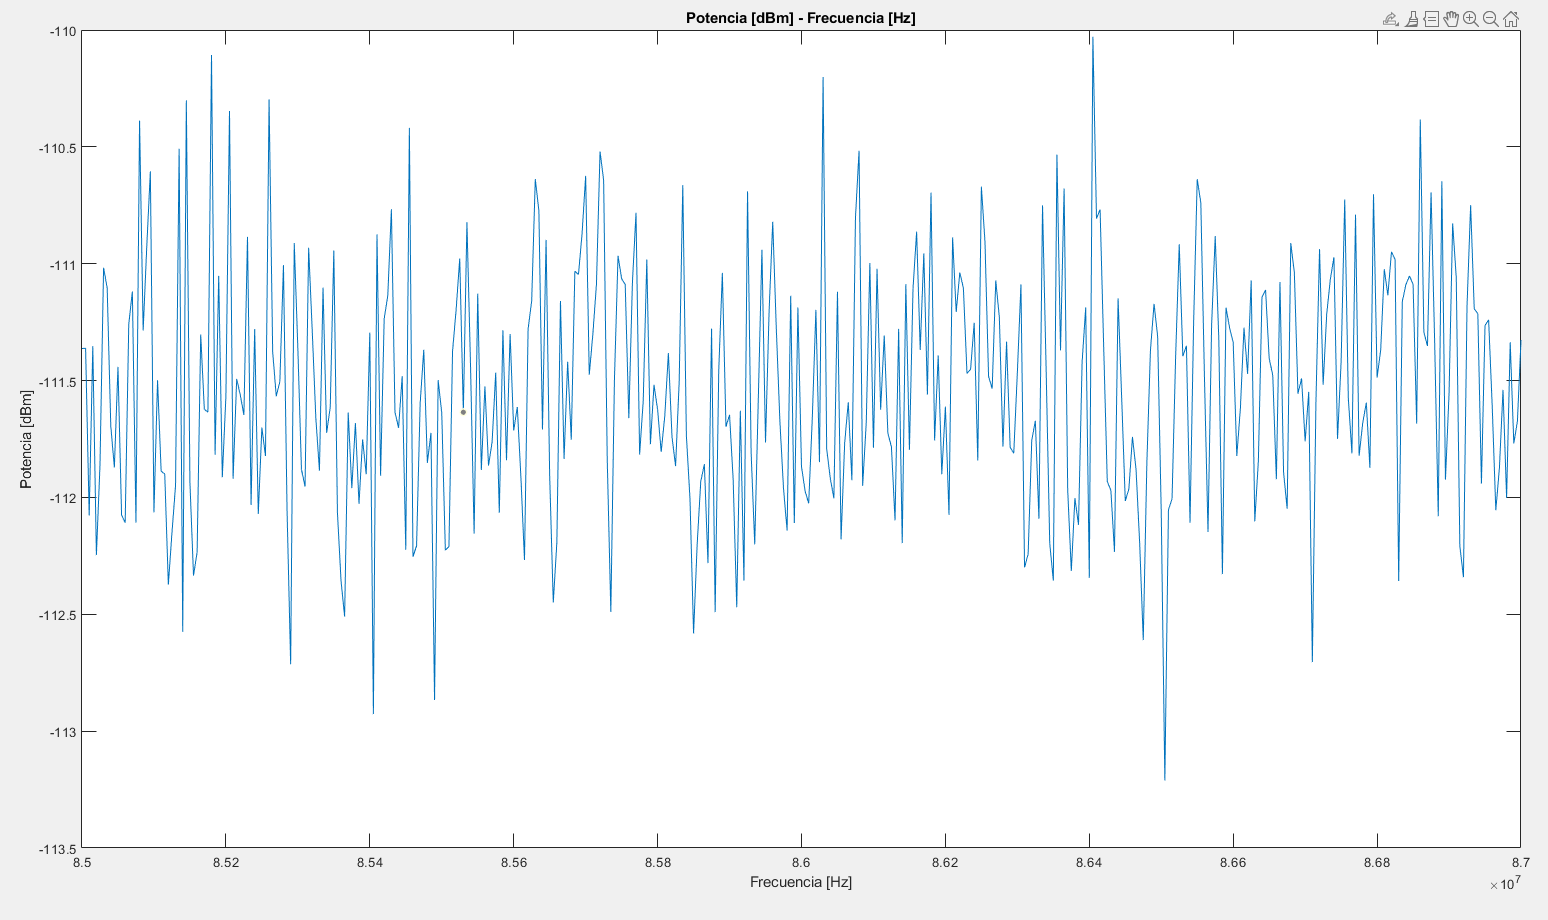
\includegraphics[width=0.5\textwidth]{media/piso-ruido}
		\caption{Piso de Ruido de una señal sin perturbación controlada}
		\label{fig:piso-ruido}
	\end{figure}
	
	Por otro lado en la figura \ref{fig:piso-ruido-disc} se puede apreciar el piso de ruido luego de aplicar un discriminador simple el cual se encargar de suprimir los sobre picos de la señal, para este caso los valores extremos de la señal se ubicaban en la parte inferior de la misma y para valores superiores a los -12dBm, finalmente limitada la señal se obtuvo la media, siendo el piso de ruido equivalente a $-111.5306 [dBm]$
	
	\begin{figure}[h]
		\centering
		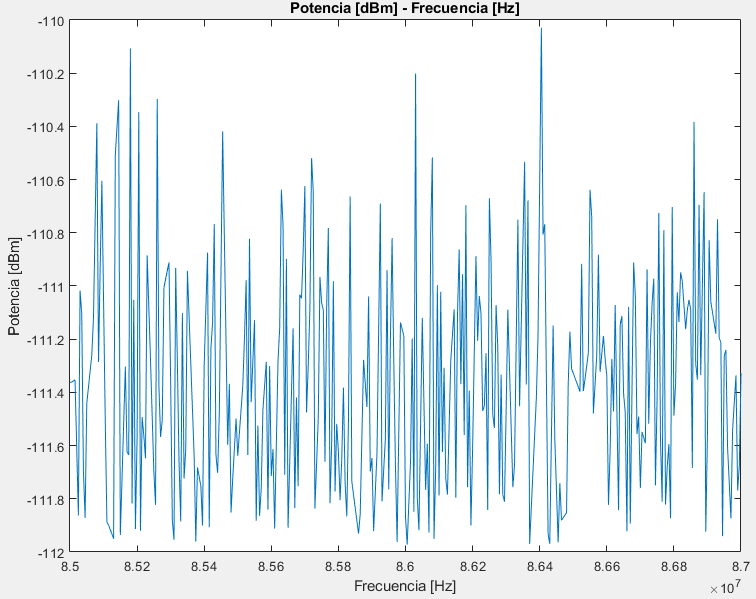
\includegraphics[width=0.5\textwidth]{media/piso-ruido-disc}
		\caption{Piso ruido discriminado}
		\label{fig:piso-ruido-disc}
	\end{figure}
	
	
	\section{Análisis de datos}
	
	En función al procedimiento para la obtención del piso de ruido este se aplico a las diferentes mediciones realizadas y su archivo de datos de salida correspondiente, para ello además la jerarquía de archivos definida ayudo con este procedimiento permitiendo analizar en caso se desee solo las señales de ruido (sin transmisión) o las señales transmitida para un determinado valor de índice de modulación $\beta$.
	
	Para este propósito se definió un bucle general con instrucciones para realizar la lectura de archivos desde la carpeta $'/data2/'$, seguidamente se realiza el ploteo de las archivos leídos y la media del nivel de ruido obtenido para cada archivo luego de aplicar el discriminador de picos.
	
	En la figura \ref{fig:seniales-ruido} se muestran un gráfica general del piso del ruido siendo afectado por el generador de ruido para las distancias entre $0cm y 250cm$, gráficas que además se tomaron como referencia para establecer un nivel umbral para el discriminador a aplicar.
	
	\begin{figure}[h]
		\centering
		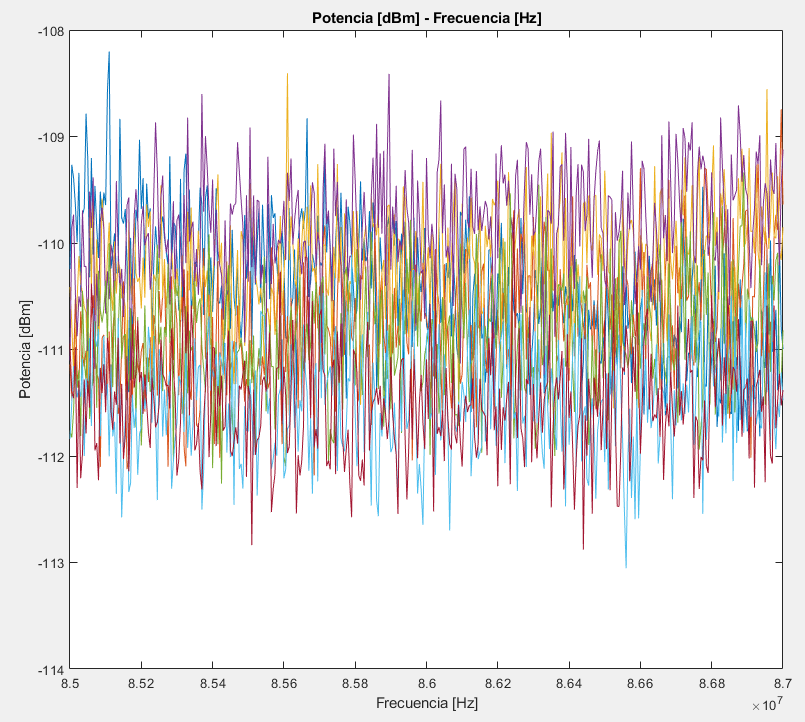
\includegraphics[width=0.5\textwidth]{media/seniales-ruido}
		\caption{Señales de ruido sin transmisión}
		\label{fig:seniales-ruido}
	\end{figure}
	
	Como resultado de este análisis se pudo apreciar que el nivel de ruido presenta sobre picos por debajo de los $-112 [dBm]$, una vez realizadas ambas acciones se ejecutaron 2 procesos por cada ciclo del bucle.
	
	\begin{enumerate}
		\item Eliminar sobrepicos mediante el discriminador
		\item Obtener la media para la señal de ruido a la salida del discriminador.
	\end{enumerate}
	
	Además al mismo tiempo se realiza una correlación entre cada media o promedio resultante con la distancia del generador de ruido al analizador de espectros con el cual se realizaron las medidas, siendo así que el primer punto y consecuentes se correlacionan con las medidas en distancia de $10, 30, 50, 100, 150, 200, 250$ cm para cada una de ellas respectivamente, el resultado de este procedimiento se puede apreciar en la figura \ref{fig:potencia-distancia}.
	
	\begin{figure}[h]
		\centering
		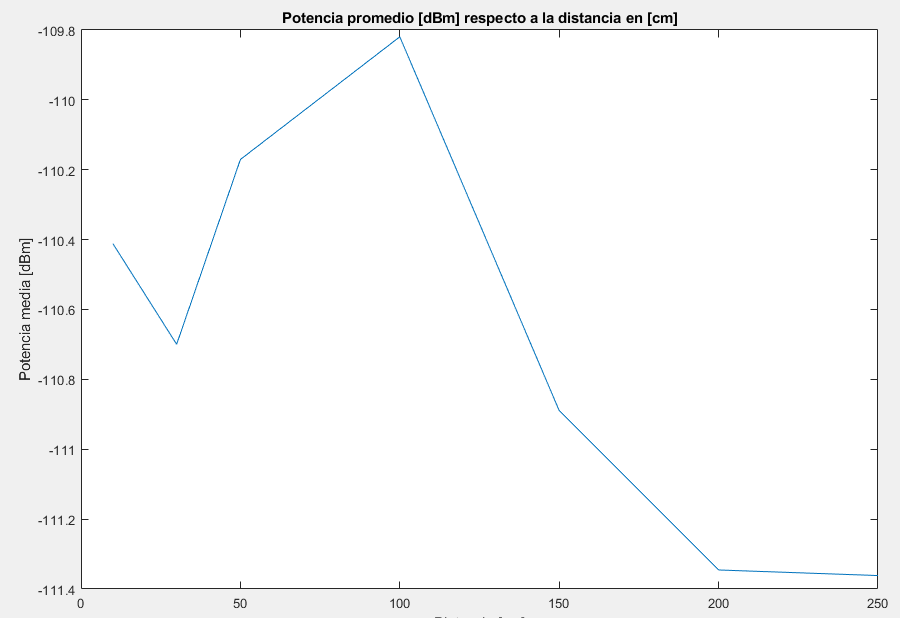
\includegraphics[width=0.5\textwidth]{media/potencia-distancia}
		\caption{Piso de ruido respecto al nivel a la distancia del generador de ruido}
		\label{fig:potencia-distancia}
	\end{figure}
	
	En la tabla \ref{tab:resumen-piso-ruido} se muestra una tabla resumen de las media obtenido para cada medición en función a la distancia.
	
	\begin{table}[]
		\centering
		\begin{tabular}{|ccc|}
			\hline
			\multicolumn{3}{|c|}{\textbf{Barrido   de frecuencias}}                                                  \\ \hline
			\multicolumn{1}{|c|}{\textbf{f (Hz)}} & \multicolumn{1}{c|}{\textbf{Vo {[}mV{]}}} & \textbf{Io {[}mA{]}} \\ \hline
			\multicolumn{1}{|c|}{10}              & \multicolumn{1}{c|}{333.437}              & 0.666875             \\ \hline
			\multicolumn{1}{|c|}{20}              & \multicolumn{1}{c|}{516.629}              & 1.033                \\ \hline
			\multicolumn{1}{|c|}{50}              & \multicolumn{1}{c|}{662.684}              & 1.325                \\ \hline
			\multicolumn{1}{|c|}{100}             & \multicolumn{1}{c|}{695.498}              & 1.391                \\ \hline
			\multicolumn{1}{|c|}{200}             & \multicolumn{1}{c|}{704.455}              & 1.409                \\ \hline
			\multicolumn{1}{|c|}{300}             & \multicolumn{1}{c|}{706.099}              & 1.412                \\ \hline
			\multicolumn{1}{|c|}{400}             & \multicolumn{1}{c|}{706.733}              & 1.413                \\ \hline
			\multicolumn{1}{|c|}{500}             & \multicolumn{1}{c|}{706.954}              & 1.414                \\ \hline
			\multicolumn{1}{|c|}{600}             & \multicolumn{1}{c|}{707.086}              & 1.414                \\ \hline
			\multicolumn{1}{|c|}{700}             & \multicolumn{1}{c|}{707.1}                & 1.414                \\ \hline
			\multicolumn{1}{|c|}{708.93}          & \multicolumn{1}{c|}{707.1}                & 1.414                \\ \hline
			\multicolumn{1}{|c|}{850}             & \multicolumn{1}{c|}{707.063}              & 1.414                \\ \hline
			\multicolumn{1}{|c|}{950}             & \multicolumn{1}{c|}{706.984}              & 1.414                \\ \hline
			\multicolumn{1}{|c|}{1000}            & \multicolumn{1}{c|}{706.939}              & 1.414                \\ \hline
			\multicolumn{1}{|c|}{1200}            & \multicolumn{1}{c|}{706.757}              & 1.414                \\ \hline
			\multicolumn{1}{|c|}{2000}            & \multicolumn{1}{c|}{705.517}              & 1.411                \\ \hline
			\multicolumn{1}{|c|}{2500}            & \multicolumn{1}{c|}{704.37}               & 1.409                \\ \hline
			\multicolumn{1}{|c|}{3500}            & \multicolumn{1}{c|}{701.313}              & 1.403                \\ \hline
			\multicolumn{1}{|c|}{5000}            & \multicolumn{1}{c|}{695.028}              & 1.39                 \\ \hline
		\end{tabular}
		\caption{Resumen: Distancia respecto al piso de ruido}
		\label{tab:resumen-piso-ruido}
	\end{table}
	
	De lo anterior se puede concluir que a 250 centímetros no existe una afectación relevante en el piso de ruido a causa del generador de ruido cuyo valor de referencia es equivalente a $-111.5306 [dBm]$ mientras que ello se va incrementando conforme la distancia se acorta entre la antena receptora, obteniendo su valor pico a los 100cm para un valor de $-109.819 [dBm]$
	
	\section{Observaciones}
	
	\begin{itemize}
		\item El uso de la media como determinante en el nivel de ruido es un proceso que se ve afectado fácilmente por valores extremos (sobre picos en la señal), por lo tanto un método alternativo podría brindar mayor certeza sin la necesidad de aumentar la complejidad computacional.
		\item A pesar de la eficiencia en el sistema de bloques definidos para la transmisión y recepción de la señal FM en GNU Radio es posible mejorar los mismos para poder modificar la mayor cantidad de parámetros como la amplitud de la señal de información, el índice de modulación, frecuencia de corte de los filtros, los cuales actualmente se definen de forma estática.
	\end{itemize}
	
	
	
	\bibliographystyle{IEEEtran}
	\bibliography{biblio}
\end{document}
